\documentclass[a4paper,12pt]{article} % тип документа
\usepackage[margin=1in]{geometry} % Поля

%  Русский язык
\usepackage[warn]{mathtext}
\usepackage[T2A]{fontenc}			% кодировка
\usepackage[utf8]{inputenc}			% кодировка исходного текста
\usepackage[english,russian]{babel}	% локализация и переносы
% Математика
\usepackage{amsmath,amsfonts,amssymb,amsthm,mathtools} 
\usepackage{wasysym}
%%%
\usepackage{graphicx}

\usepackage{tabularx}

\usepackage{gensymb} % знак градуса
\usepackage{enumitem} % изменить список enumerate
\usepackage{placeins} % \FloatBarrier

\renewcommand{\thesection}{\Roman{section}} 
\renewcommand{\thesubsection}{\roman{subsection}}


\begin{document}

\newcolumntype{Y}{>{\centering\arraybackslash}X} %new tabularx


%титул
\hrule 	
\medskip
\begin{raggedright}
{\large \textbf{Вопрос по выбору по курсу общей физики на тему:}}
\\
\medskip
{\Large Атмосферные оптические явления связанные с отражением, преломлением, дисперсией и дифракцией света на распылённых в атмосфере частицах воды и льда.} 
\\
\medskip
{\large Карташов Констанин Б04-005}
\medskip
\hrule
\medskip
\end{raggedright}


\section{Оптические явления вызванные распылёнными в атмосфере каплями воды}

\subsection{Радуга}


\paragraph{} В качестве простейшей модели радуги, рассмотрим распылённые в воздухе капли воды имеющие форму идеальной сферы. Будем считать что солнечный свет -- плоская волна неполяризованного белого света. Рассмотрим каплю воды в осевом сечении. Построим ход пучка параллельных лучей падающего на каплю, заметим, что угол между отражённым и падающим лучом не превышает некоторого $ \theta_{\max} $, подобного минимальному углу отклонения в призме. Будем считать, что свет отражённый под этим углом будет иметь наибольшую интенсивность.

\begin{figure}[h]
\centering
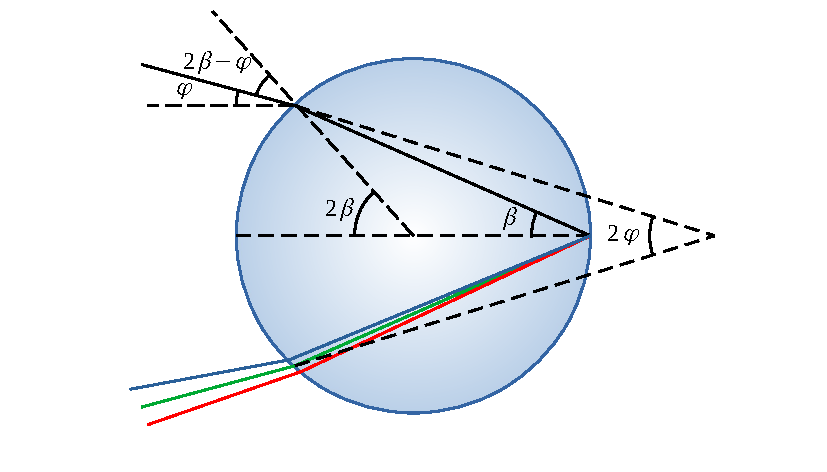
\includegraphics[width=0.7\textwidth]{dropmath.pdf}
\caption{Путь луча прошедшего через сферическую каплю воды}
\label{fig:dropmath}
\end{figure}


\paragraph{} Найдём угол $\theta_{\max}$. Для этого выделим ось капли являющейся нормалью точки в которой происходит внутренне отражение в капле. Обозначим углы $\beta$ -- угол падения луча внутри капли, $\varphi$ -- угол между осью капли и внешним падающим лучом, тогда угол отражения луча $\theta = 2 \varphi$ (рис. \ref{fig:dropmath}). Из закона Снеллиуса найдём:

\begin{equation}
\sin{(2 \beta - \varphi)} = n \sin{\beta} \; \Rightarrow \; \varphi = 2\beta - \arcsin{(n \sin{\beta})}.
\label{e:snell}
\end{equation}

\noindent Найдём $\beta_{\max}$ из условия $ d\varphi / d\beta = 0$:

\begin{equation}
\frac{d\varphi}{d\beta} = 2 - \frac{n \cos{\beta}}{\sqrt{1 - n^2 \sin^2 \beta}} = 0 \; \Rightarrow \;
\beta_{\max} = \arcsin{\frac{ \sqrt{4 - n^2}}{n\sqrt{3}}},
\label{e:betamax}
\end{equation}

\noindent подставляя (\ref{e:betamax}) в (\ref{e:snell}) получим:

\begin{equation}
\theta_{\max} = 2 \varphi_{\max} = 4 \arcsin{\frac{ \sqrt{4 - n^2}}{n\sqrt{3}}} - 2 \arcsin{n\frac{ \sqrt{4 - n^2}}{n\sqrt{3}}}.
\label{e:thetamax}
\end{equation}

\noindent Подставим в (\ref{e:thetamax}) несколько значений показателя преломления $n$: для красной длины волны $\lambda_{\text{кр}} = 750$ нм $n_{\text{кр}} = 1.330$, получаем $\theta_{\max, \text{кр}} = 42.5 \degree$, для зелёной длины волны $\lambda_{\text{зел}} = 550$ нм $n_{\text{зел}} = 1.333$, получаем $\theta_{\max, \text{зел}} = 42.1 \degree$, для синей длины волны $\lambda_{\text{син}} = 450$ нм $n_{\text{син}} = 1.337$, получаем $\theta_{\max, \text{син}} = 41.5 \degree$.

\paragraph{}В силу осевой симметрии, свет отражённый таким образом каплей воды, будет иметь вид конуса с углом $2\theta_{\max}$ на вершине. Теперь учтём большое количество капель: получим множество плоских волн, распространяющихся под углом  $\theta_{\max}$ к направлению падения солнечных лучей. Наблюдатель в таком случае будет видеть мнимое изображения разноцветного кольца находящегося на бесконечном расстоянии от него, с угловым радиусом $\theta_{\max} \approx 42 \degree$, причём с наружу кольцо будет красным, а изнутри синем. Учтём также, что свет отражённый подобным образом не может быть отражён под углом большим, чем $\theta_{\max}$, поэтому внутренность кольца будет заметно светлее внешней части.  \ref{fig:double-rainbow}.


\subsection{Двойная радуга}

\paragraph{} В прошлом пункте рассматривалось одноразовое внутренне отражение в сферической капле, однако возможны и случаи многократного внутреннего отражения. Наиболее часто наблюдаемым является случай двойного отражения. Отличие этого случая от прошлого в том, что угол между отражённым и падающими лучами будет не менее $\theta_{\min}$.

\begin{figure}[h]
\centering
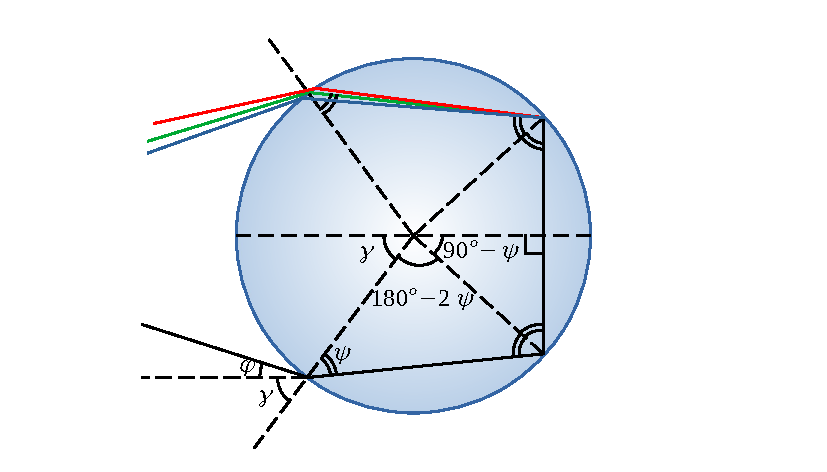
\includegraphics[width=0.7\textwidth]{dropmath2.pdf}
\caption{\centering Путь луча прошедшего через сферическую каплю воды с двойным внутренним отражением}
\label{fig:dropmath2}
\end{figure}

\paragraph{} Найдём $\theta_{\min}$.Обозначим углы $\psi$ -- угол падения луча внутри капли, $\gamma$ -- дополнительный угол для построения, $\varphi$ -- угол между осью капли и внешним падающим лучом, тогда угол отражения луча $\theta = 2 \varphi$ (рис. \ref{fig:dropmath}). Из закона Снеллиуса найдём:

\begin{equation}
\varphi = \arccos(-n \sin{\psi}) - 3 \psi.
\label{e:snell2}
\end{equation}

\noindent Из условия $d\varphi / d\psi = 0$ найдём $\psi_{\min}$:

\begin{equation}
\psi_{\min} = \arcsin{\frac{\sqrt{9 - n^2}}{2\sqrt{2} n}}.
\label{e:psimin}
\end{equation}

\noindent Подставляя (\ref{e:psimin}) в (\ref{e:snell2}) получим:

\begin{equation}
\theta_{\min} = 2 \varphi_{\min} = 2 \arccos{\frac{-\sqrt{9 - n^2}}{2\sqrt{2}}} - 6 \arcsin{\frac{\sqrt{9 - n^2}}{2\sqrt{2}n}}.
\label{e:thetamin1}
\end{equation}

\noindent Подставим в (\ref{e:thetamin1}) несколько значений показателя преломления $n$: для красной длины волны $\lambda_{\text{кр}} = 750$ нм $n_{\text{кр}} = 1.330$, получаем $\theta_{\min, \text{кр}} = 50.1 \degree$, для зелёной длины волны $\lambda_{\text{зел}} = 550$ нм $n_{\text{зел}} = 1.333$, получаем $\theta_{\min, \text{зел}} = 50.9 \degree$, для синей длины волны $\lambda_{\text{син}} = 450$ нм $n_{\text{син}} = 1.337$, получаем $\theta_{\min, \text{син}} = 51.9 \degree$.

\paragraph{} Аналогично с предыдущим пунктом, наблюдатель будет видеть мнимое изображение кольца находящегося на бесконечности. При этом угловой радиус кольца будет $\theta_{\min} \approx 51 \degree$, при этом внутренняя сторона кольца будет красной, а внешняя -- синей. Также внутренность кольца будет темнее внешности. Фото явления на рис. \ref{fig:double-rainbow}.

\begin{figure}[h]
\centering
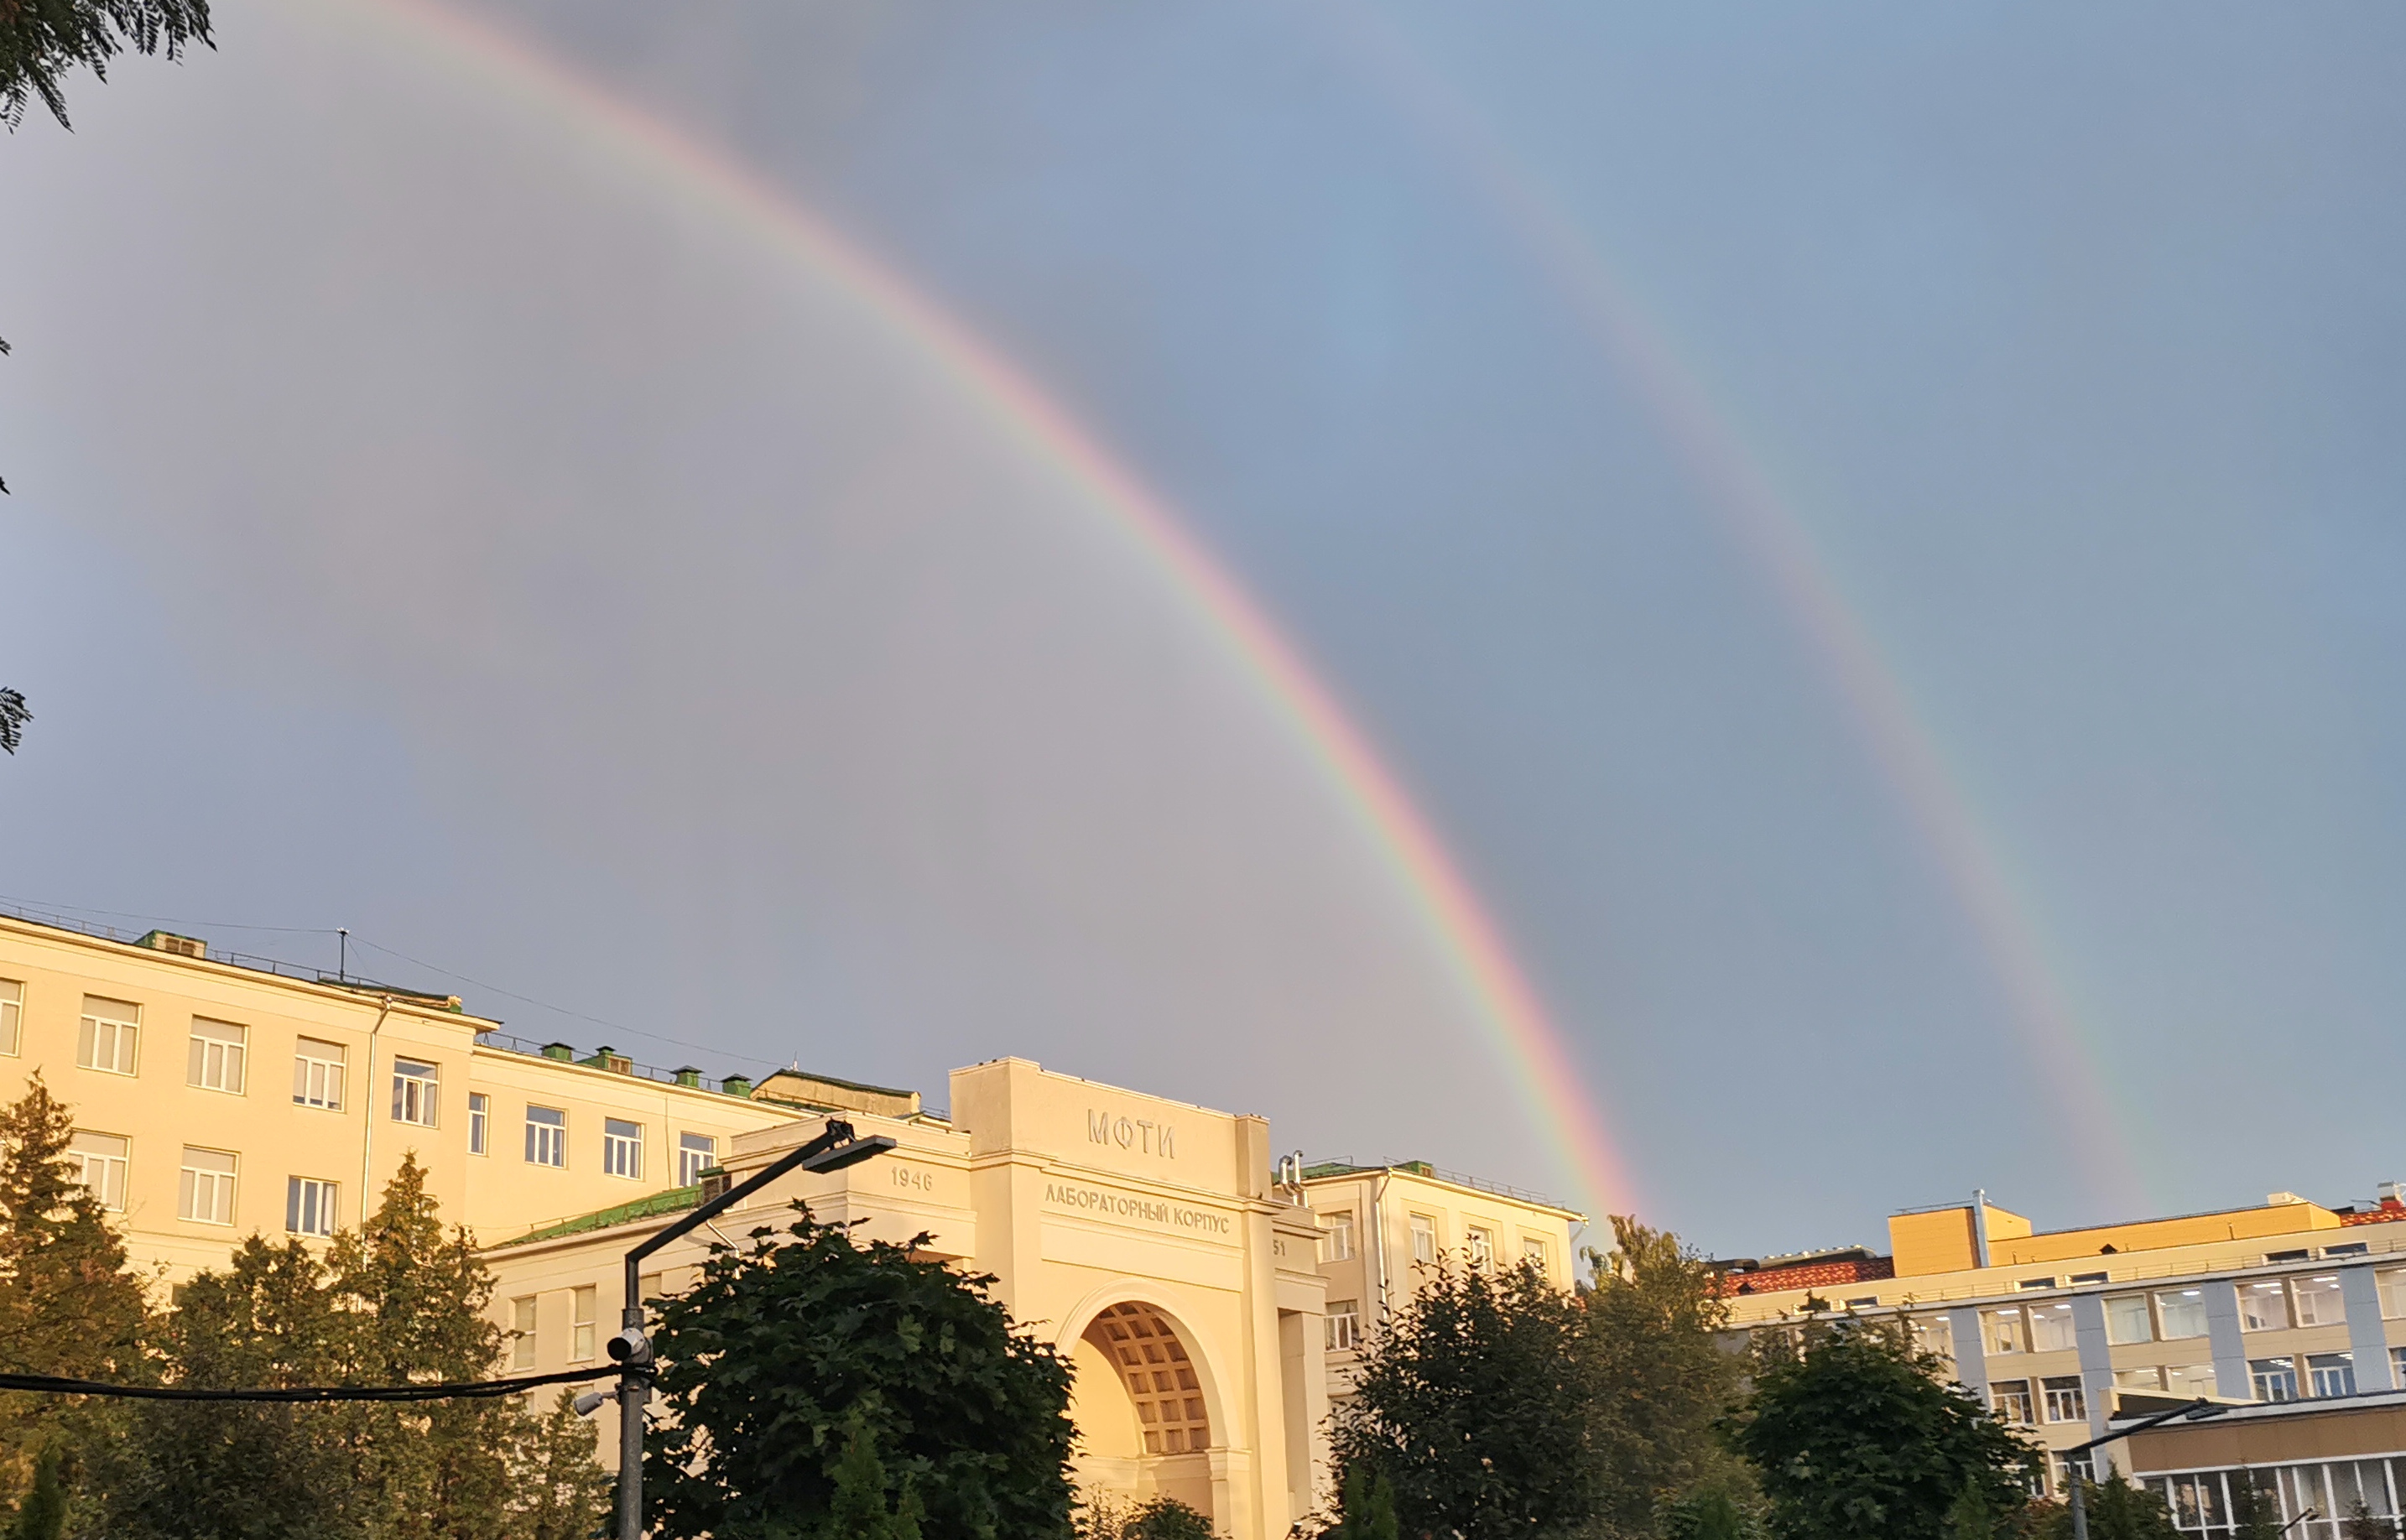
\includegraphics[width=0.7\textwidth]{double_rainbow2.jpg}
\caption{Фото двойной радуги, автор фото: Карташов Константин}
\label{fig:double-rainbow}
\end{figure}


\subsection{Корона и Глория}

\paragraph{} Другое атмосферное явление, связанное с дифракцией света может наблюдаться при распылении в воздухе мелких сферических капель с одинаковыми радиусами $r \sim 5$ мкм.

\paragraph{} При падении света на мелкую каплю воды, можно наблюдать дифракцию Фраунгофера. Как известно, дифракционная картина при дифракции Фраунгофера не зависит от расстояния на котором производится наблюдение: максимумы и минимумы дифракции имеют постоянный угловой размер. 

\paragraph{} Учитывая большое количество капель, получим, что наблюдатель будет видеть дифракционную картину (диск Эйри), расположенный на бесконечности, с угловым радиусом первого максимума $\theta \sim \frac{\lambda}{r} \approx 5 \degree$. При этом, если дифракционная картина образована светом идущего непосредственно от солнца, то в центре колец будет находится солнце -- такое явление называется короной. Если же дифракционная картина образована светом отражённым в обратном направлении -- это явление будет называться Глорией, Брокенским призраком или светом Будды. Фото явления на рис. \ref{fig:glory}.

\begin{figure}[h]
\centering
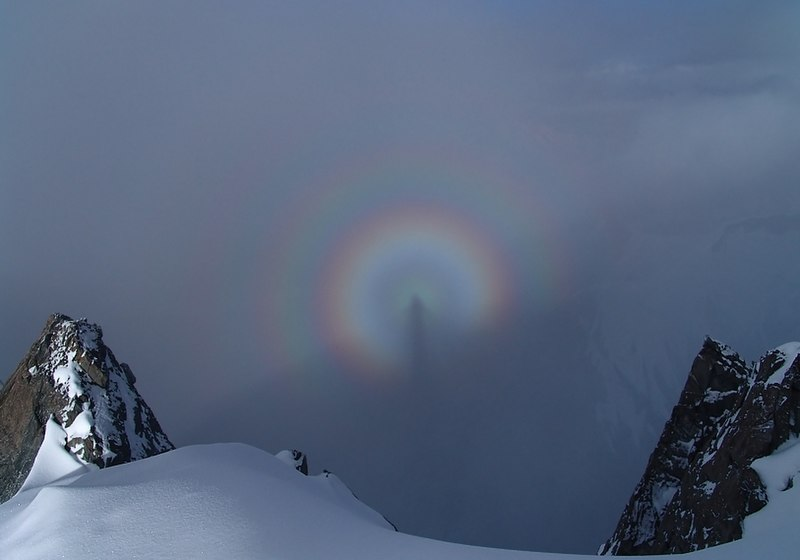
\includegraphics[width=0.7\textwidth]{glory_dmitry_shapovalov.jpg}
\caption{Эффект брокенского призрака, автор фото: Дмитрий Шаповалов}
\label{fig:glory}
\end{figure}

\medskip\hrule\medskip

\section{Оптические явления вызванные распылёнными в атмосфере частицами льда}

\subsection{Гало}

\paragraph{} Как известно, кристалл льда имеет структуру правильной шестиугольной призмы, будем читать что частицы для распылённые в воздухе будут иметь такую же структуру. Для объяснения феномена гало рассмотрим преломление лучей в плоскости параллельной основанию кристаллика льда. Здесь возможны три случая преломления (рис. \ref{fig:iceprism}): 

\begin{enumerate}
\item Луч заходит в сторону кристалла, претерпевает полное внутреннее отражение от соседней стороны, и выходит из кристалла. Этот случай нас не интересует, так как равносилен отражению от зеркала со случайной ориентацией.
\item Луч заходит в сторону кристалла и выходит из из стороны находящейся под углом $\alpha = 60\degree$ к первой. Это равносильно прохождению света через призму в виде равностороннего треугольника. 
\item Луч заходит в сторону кристалла и выходит из противоположной стороны. Этот случай нас не интересует.
\end{enumerate}

\begin{figure}
\centering
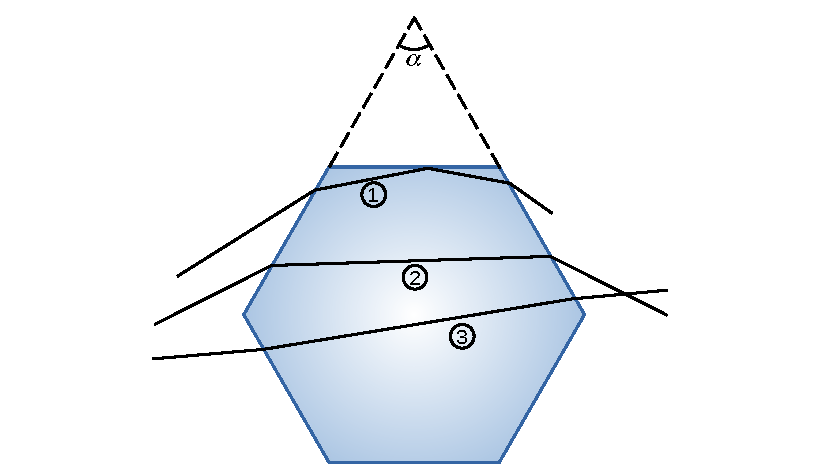
\includegraphics[width=0.7\textwidth]{iceprism.pdf}
\caption{Пути преломления в сечении кристаллика льда}
\label{fig:iceprism}
\end{figure}

\paragraph{} Заострим внимание на втором случае. При прохождении рассеянного света через призму, наибольшая интенсивность будет у света прошедшего близко к углу наименьшего преломления $\theta_{\min}$. Из известного для призмы соотношения получаем:

\begin{equation}
\frac{\sin{\dfrac{\alpha + \theta_{\min}}{2}}}{\sin{\dfrac{\alpha}{2}}} = n \; \Rightarrow \theta_{\min} = 2 \arcsin{\left( n \sin{\frac{\alpha}{2}} \right)} - \alpha
\label{e:thetamin}
\end{equation} 

\noindent Подставим в (\ref{e:thetamin}) несколько значений показателя преломления $n$: для красной длины волны $\lambda_{\text{кр}} = 750$ нм $n_{\text{кр}} = 1.306$, получаем $\theta_{\min, \text{кр}} = 21.5 \degree$, для синей длины волны $\lambda_{\text{син}} = 350$ нм $n_{\text{син}} = 1.325$, получаем $\theta_{\min, \text{син}} = 23.0 \degree$.

\paragraph{} Солнечный свет, падающий на кристаллики льда не является рассеянным, поэтому от каждого кристаллика свет будет преломлён под углом $\theta \geq \theta_{\min}$. Пусть распылённые в воздухе кристаллики имеют случайную ориентацию, тогда сумма преломлённых волн будет равносильна плоским волнам, распространяющихся под углом $\theta$ к направлению распространения света идущего от солнца, причём волны распространяющиеся под углом $\theta_{\min}$ будут иметь наибольшую интенсивность. Наблюдатель будет видеть мнимое изображение яркого кольца находящегося на бесконечности с угловым радиусом $\theta_{\min} \approx 22 \degree$, причём внутренний край кольца будет красноватым, а внешний край -- синеватым. При этом внутренность кольца будет заметно темнее внешности, так как свет не преломляется под углом меньшим $\theta_{\min}$. Фото явления на рис. \ref{fig:halo_1}.

\begin{figure}[h]
\centering
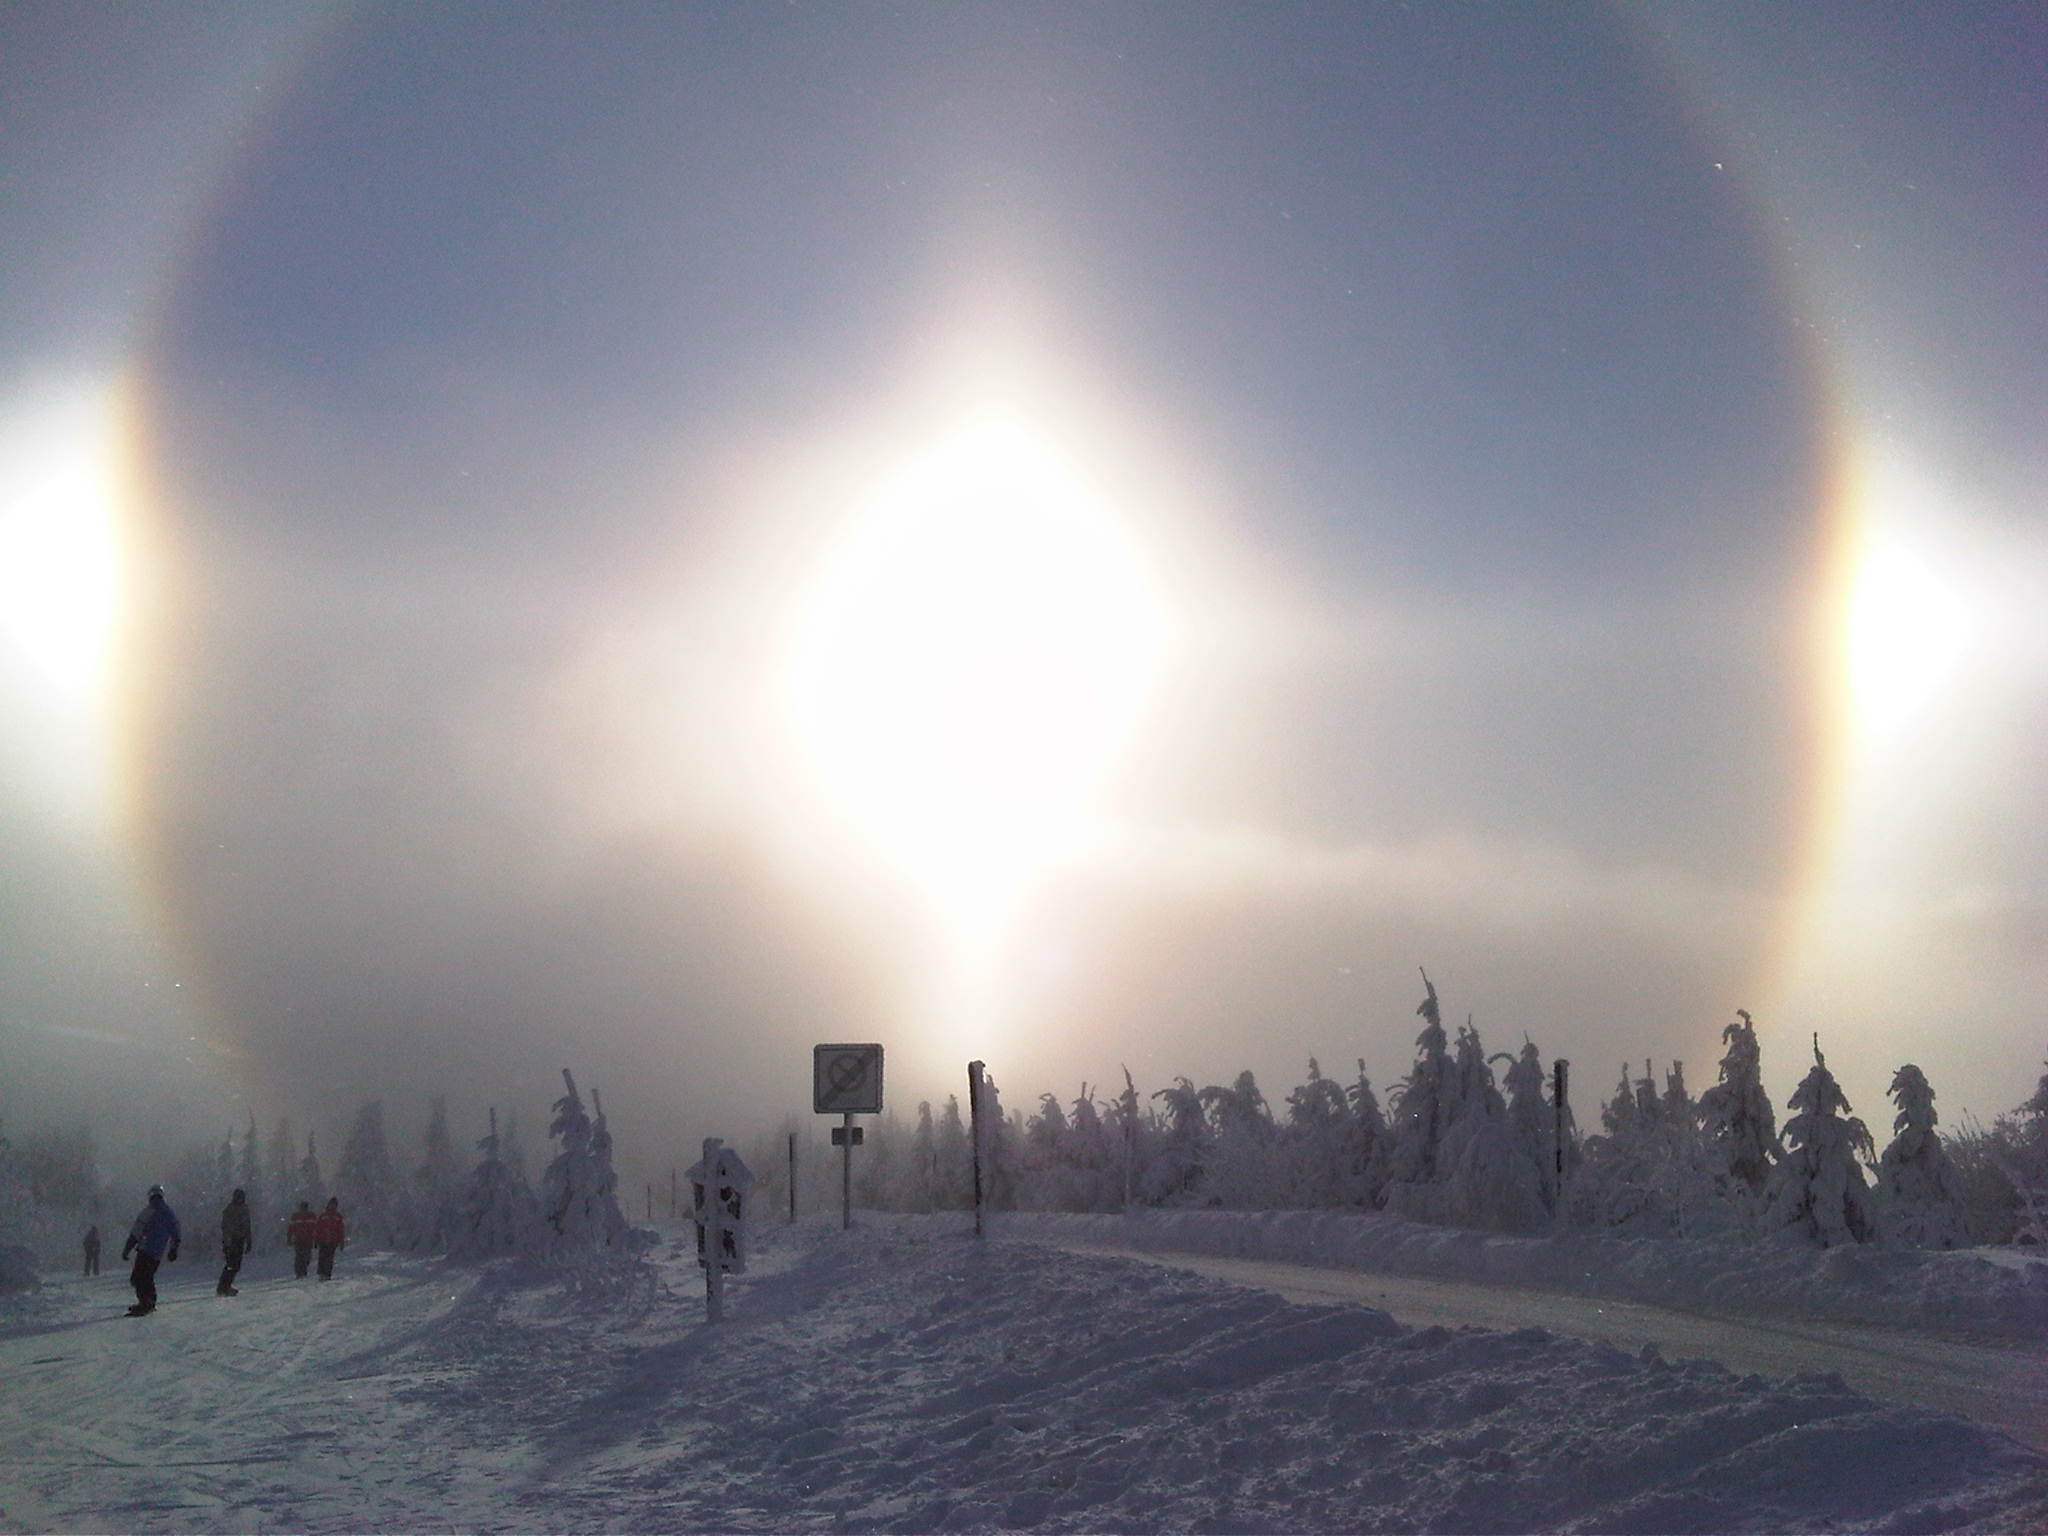
\includegraphics[width=0.7\textwidth]{halo_1.jpg}
\caption{Гало с паргелием, автор фото: Карташов Константин}
\label{fig:halo_1}
\end{figure}



\subsection{Вторичное гало}

\paragraph{} Проводя такие же рассуждения как в предыдущем пункте, рассмотрим преломление в плоскости перпендикулярной основанию кристаллика льда. Сечение кристалла в этой плоскости будет иметь вид прямоугольника, поэтому возможны два случая преломления (рис. \ref{fig:iceprism2}):

\begin{figure}
\centering
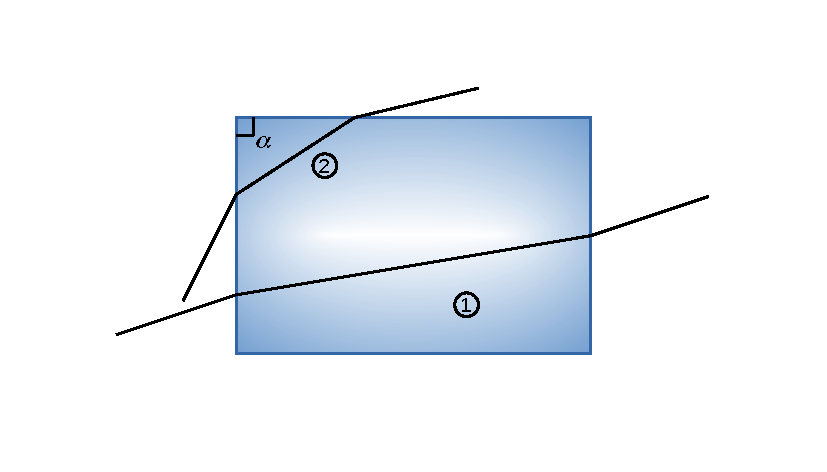
\includegraphics[width=0.7\textwidth]{iceprism2.pdf}
\caption{Пути преломления в сечении кристаллика льда}
\label{fig:iceprism2}
\end{figure}

\begin{enumerate}
\item Луч проходит через противоположные грани. Этот случай нас не интересует.
\item Луч преломляется на грани и основании. В этом случае кристаллик будет играть роль призмы с углом $\alpha = 90\degree$.
\end{enumerate}

\paragraph{} Во втором случае получим изображение с такими же свойствами, как в предыдущем пункте, при этом $\theta_{\min} \approx 46 \degree$. 

\begin{figure}[h]
\centering
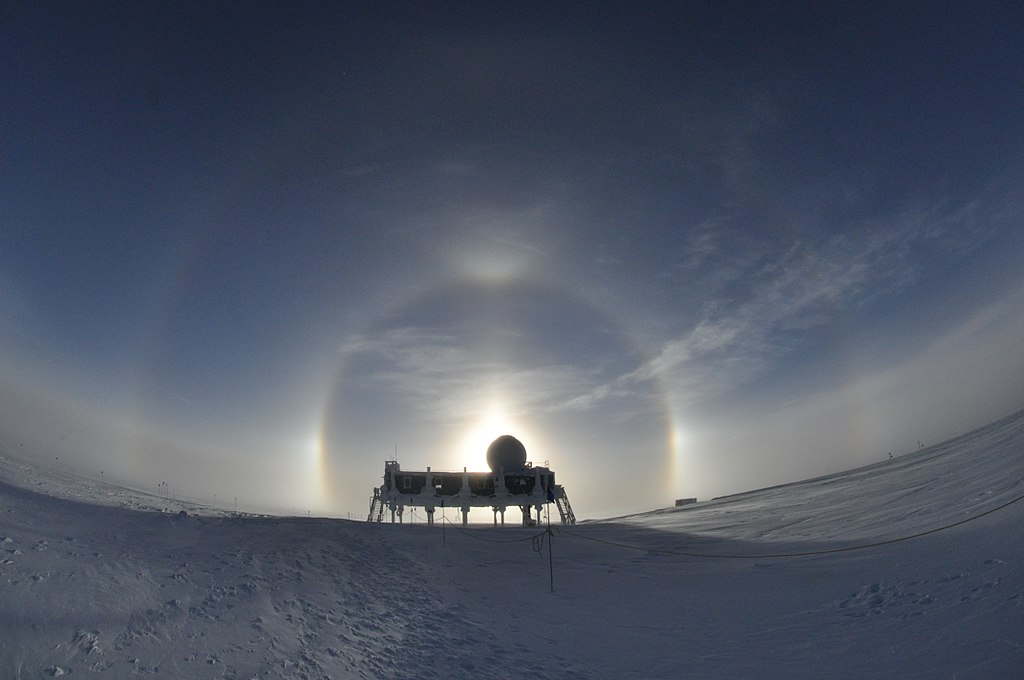
\includegraphics[width=0.7\textwidth]{halo_2.jpg}
\caption{\centering Гало со вторичным гало, автор фото: Национальное управление океанических и атмосферных исследований США}
\label{fig:halo_2}
\end{figure}

\subsection{Световой столб и паргелий}

\paragraph{} В предыдущих двух пунктах рассматривался случай, когда кристаллики льда расположены в случайных ориентациях. Однако обычно для разных форм кристаллов льда преобладают особые ориентации, например плоские кристаллы в форме правильной шестиугольной призмы, у которых размер основания значительно больше высоты, за счёт своих аэродинамических свойств, расположены так, что их основание параллельно поверхности земли. 

\paragraph{} При преломлении света через боковые грани таких кристаллов, свет проходит проходит так же как при образовании гало, однако из-за ориентации кристаллов, усиливаются те части гало, которые находятся на той же угловой высоте, что и солнце. Получается эффект подобный наблюдению солнца через бипризму (паргелий). (рис. \ref{fig:halo_1} и \ref{fig:halo_2})

\paragraph{}  При отражении света от оснований кристаллов расположенных основаниями параллельно к поверхности, в воздухе образуются зеркальные слои, отражающие свет распространяющийся вверх обратно вниз (схематично на рис. \ref{fig:pillar1}). Этот эффект вызывает появление над и под источником света мнимого изображения светящегося столба, имеющего такой же цвет как и источник. Особенно эффектно выглядит такой эффект, когда он вызван искусственными источниками освещения (рис. \ref{fig:pillar2})
\begin{figure}
\centering
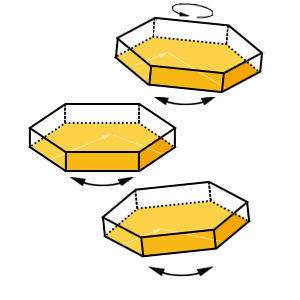
\includegraphics[width=0.3\textwidth]{light_pillar.png}
\caption{\centering Отражение света от кристаллов, вызывающие появление световых столбов}
\label{fig:pillar1}
\end{figure}

\begin{figure}
\centering
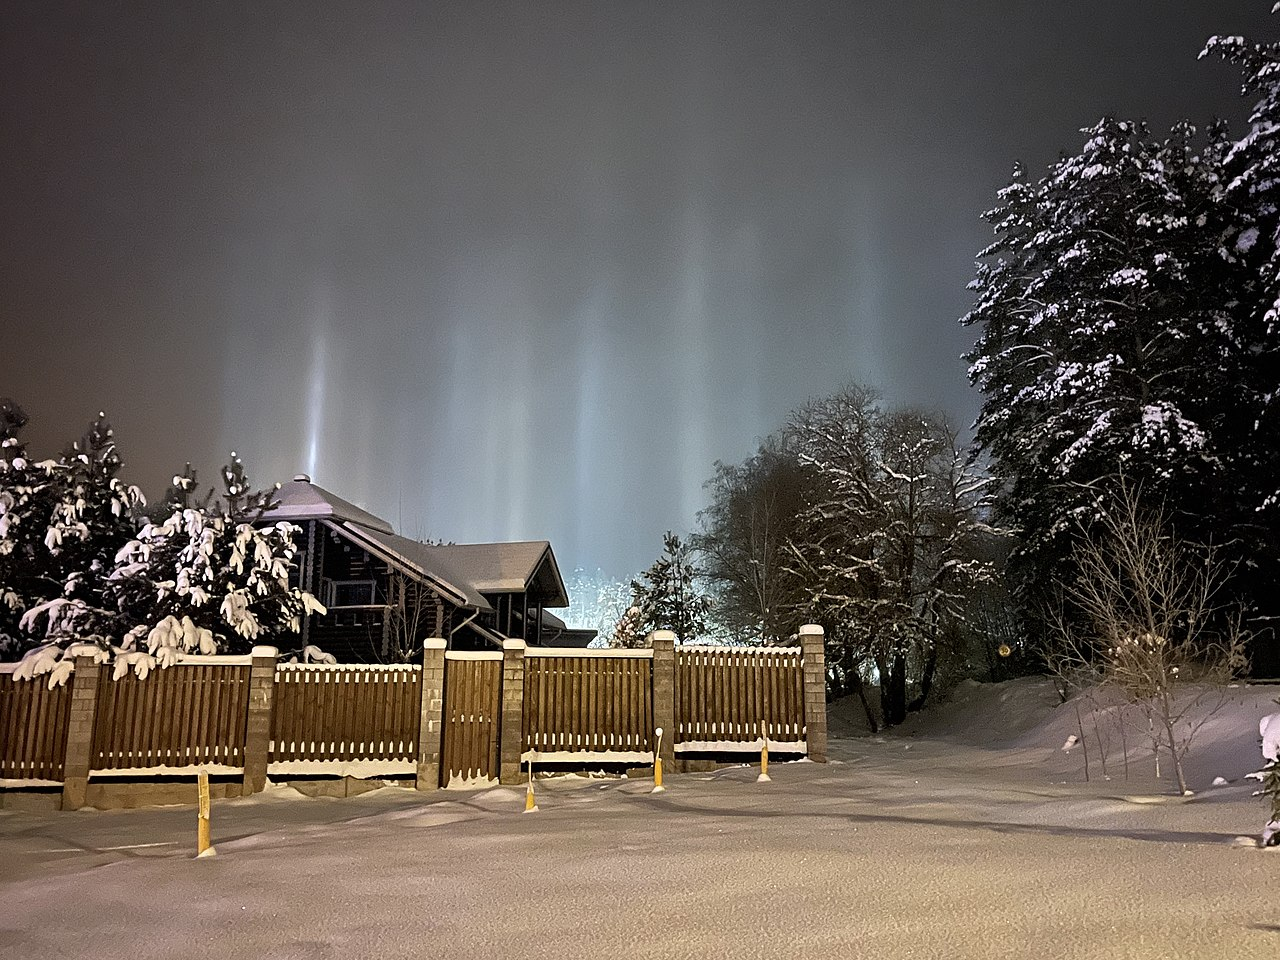
\includegraphics[width=0.7\textwidth]{light_ray.jpg}
\caption{\centering Световые столбы вызванные искусственными источниками освещения, автор фото: Дмитрий Супонау}
\label{fig:pillar2}
\end{figure}
\medskip\hrule\medskip


\end{document}
